\documentclass{article}

\usepackage{booktabs}
\usepackage{tabularx}
\usepackage{hyperref}
\usepackage{graphicx}
\usepackage{pdflscape}

\hypersetup{
    colorlinks=true,       % false: boxed links; true: colored links
    linkcolor=red,          % color of internal links (change box color with linkbordercolor)
    citecolor=green,        % color of links to bibliography
    filecolor=magenta,      % color of file links
    urlcolor=cyan           % color of external links
}

\title{Hazard Analysis\\\progname}

\author{\authname}

\date{}

%% Comments

\usepackage{color}

\newif\ifcomments\commentstrue %displays comments
%\newif\ifcomments\commentsfalse %so that comments do not display

\ifcomments
\newcommand{\authornote}[3]{\textcolor{#1}{[#3 ---#2]}}
\newcommand{\todo}[1]{\textcolor{red}{[TODO: #1]}}
\else
\newcommand{\authornote}[3]{}
\newcommand{\todo}[1]{}
\fi

\newcommand{\wss}[1]{\authornote{blue}{SS}{#1}} 
\newcommand{\plt}[1]{\authornote{magenta}{TPLT}{#1}} %For explanation of the template
\newcommand{\an}[1]{\authornote{cyan}{Author}{#1}}

%% Common Parts

\newcommand{\progname}{REVITALIZE} % PUT YOUR PROGRAM NAME HERE
\newcommand{\authname}{Team 13, REVITALIZE
\\ Bill Nguyen
\\ Syed Bokhari
\\ Hasan Kibria
\\ Youssef Dahab
\\ Logan Brown
\\ Mahmoud Anklis} % AUTHOR NAMES                  

\usepackage{hyperref}
    \hypersetup{colorlinks=true, linkcolor=blue, citecolor=blue, filecolor=blue,
                urlcolor=blue, unicode=false}
    \urlstyle{same}
                                


\begin{document}

\maketitle
\thispagestyle{empty}

~\newpage

\pagenumbering{roman}

\begin{table}[hp]
\caption{Revision History} \label{TblRevisionHistory}
\begin{tabularx}{\textwidth}{llX}
\toprule
\textbf{Date} & \textbf{Developer(s)} & \textbf{Change}\\
\midrule
October 15th, 2022 & Bill Nguyen & FMEA \\
... & ... & ...\\
\bottomrule
\end{tabularx}
\end{table}

~\newpage

\tableofcontents

~\newpage

\pagenumbering{arabic}

\wss{You are free to modify this template.}

\section{Introduction}

\wss{You can include your definition of what a hazard is here.}

\section{Scope and Purpose of Hazard Analysis}

\section{System Boundaries and Components}

\section{Critical Assumptions}

\wss{These assumptions that are made about the software or system.  You should
minimize the number of assumptions that remove potential hazards.  For instance,
you could assume a part will never fail, but it is generally better to include
this potential failure mode.}

\section{Failure Mode and Effect Analysis}
The next pages will show the full failure mode and effect analysis (FMEA) for REVITALIZE:
\begin{landscape}
\begin{figure}[ht]
	\centering
	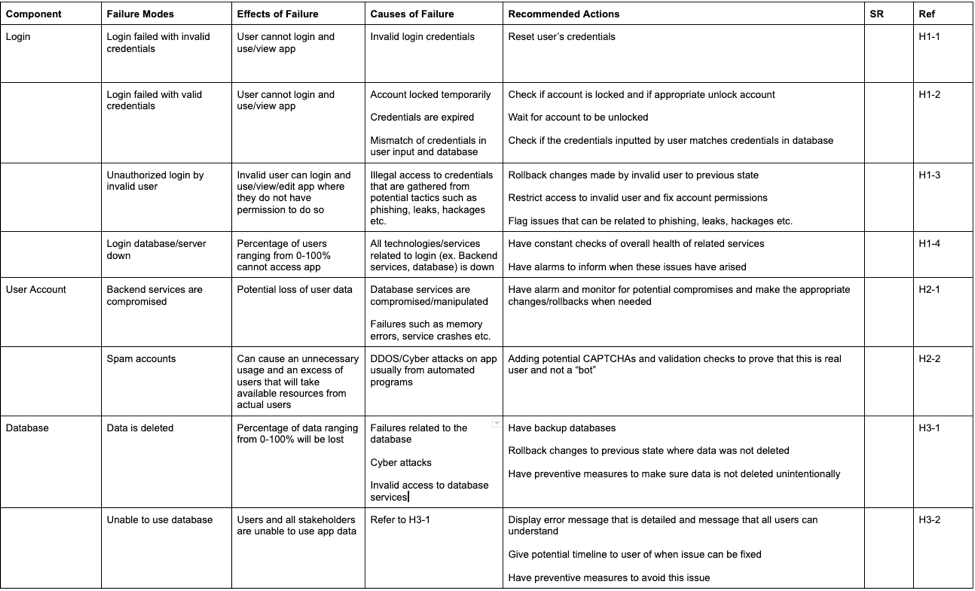
\includegraphics[angle=360, scale=1.42]{FMEAPart1.png}
	\caption{Part 1 of FMEA}
\end{figure}
\end{landscape}

\section{Safety and Security Requirements}

\wss{Newly discovered requirements.  These should also be added to the SRS.  (A
rationale design process how and why to fake it.)}

\section{Roadmap}

\wss{Which safety requirements will be implemented as part of the capstone timeline?
Which requirements will be implemented in the future?}

\end{document}